\section{Use of the Higgs Combine Tool}
\label{combine_tool}

%
% Ouline:
% - General Description of usage of Combine
% - InputFormat: Datacards and Workspaces
% - Playing with Asimov
% - Expected Limits
% - Maxlikelihood Fits
%

To perform statistical tests in order to extract physical quantities of
interest, we employ Higgs Combination Package. It allows us to perform the
tests for each category individually and to combine all categories
simultaneously as well. Given that we are performing a search of SM Higgs
boson, the main objective is to improve (lower) the expected exclusion limits
that we are to put on SM Higgs production cross-section with the data
collected during Run~II in 2016.

\subsection{Datacards and Workspaces}
The Higgs Combination Package uses datacards and workspaces where models
are defined to perform the tests. A datacard outlines our models, yields
from data, signal and background processes. In the datacard, we also list all
of uncertainties (nuisances) that can modify the yields of our models.
Workspaces are the containers for the programmatically specified signal and
background models. The detailed list of inputs that are used in the combination
 is the following:

\begin{itemize}
    \item Mass shapes for data for each category.
    \item Background models for each category. All of models come inside of
an envelope (RooMultiPdf) as described in Sec.~\ref{bkg_model}. The overall
normalization for the background yield as well as the parameters of each
functional form are floating, as described in Sec.~\ref{bkg_model}.  %and constrained by the Combination Package once the fit is performed.
    \item Signal models for each category and for each production process. All
model parameters come in as functions of the Higgs mass, as described in
Sec.~\ref{sig_model} %Given that we are performing a search,
Several Higgs mass hypotheses are tested.
% The overall normalization is frozen, however as a function of Higgs Mass.
    \item Nuisances (systematic uncertainties) that influence our
measurement (integrated luminosity, pile-up, etc...) have to be considered.
Therefore we provide multiplicative nuisance parameters that can modify the
signal yield. The systematic uncertainties are described in Sec.~\ref{sig_syst}.
\end{itemize}

\subsection{Validity Tests against Asimov}
The very first test of the validity of the model to be used is to perform the
tests against the Asimov Dataset. The tests performed can summarized in the
following procedure:

\begin{itemize}
    \item Given signal and background models we generate an Asimov dataset with
 a certain signal strength (typically 1).
    \item Performing the signal plus background fit to this Asimov dataset,
this should return back the expected signal strength that was injected in
the generation.
    %\item If a substantial bias has been observed, we can try profiling the likelihood (it's Negative Log-Likelihood to be exact) to see where the minimum of our test statistics is.
\end{itemize}

Figure~\ref{combine:AsimovTests} provides examples of testing against Asimov
dataset. The mass spectrum shown on the left side of the figure shows the
generated dataset overlaid with the fit. On the right side, the
likelihood profiling vs. the signal strength returning the injected strength
can be seen.
%In the middle and on the right, examples of likelihood profiling vs the signal strength for respectively a bad (bias)/good model.
%Important to point out that in the middle we have an example of a situation described previously - we observe a substantial amount of bias returned back from the fit of the Asimov generated with the injected signal strength of 1.
%The difference between middle and right is the granularity of the binning or number of points that are used to constrain the fit.

\begin{figure}[hbp]
     \centering
     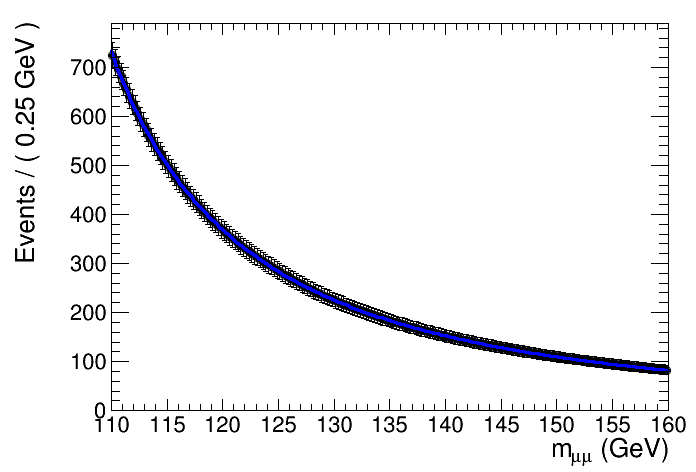
\includegraphics[width=0.475\textwidth]{figures/combine/asimovTests/cat6_x_fit_b.png}
     %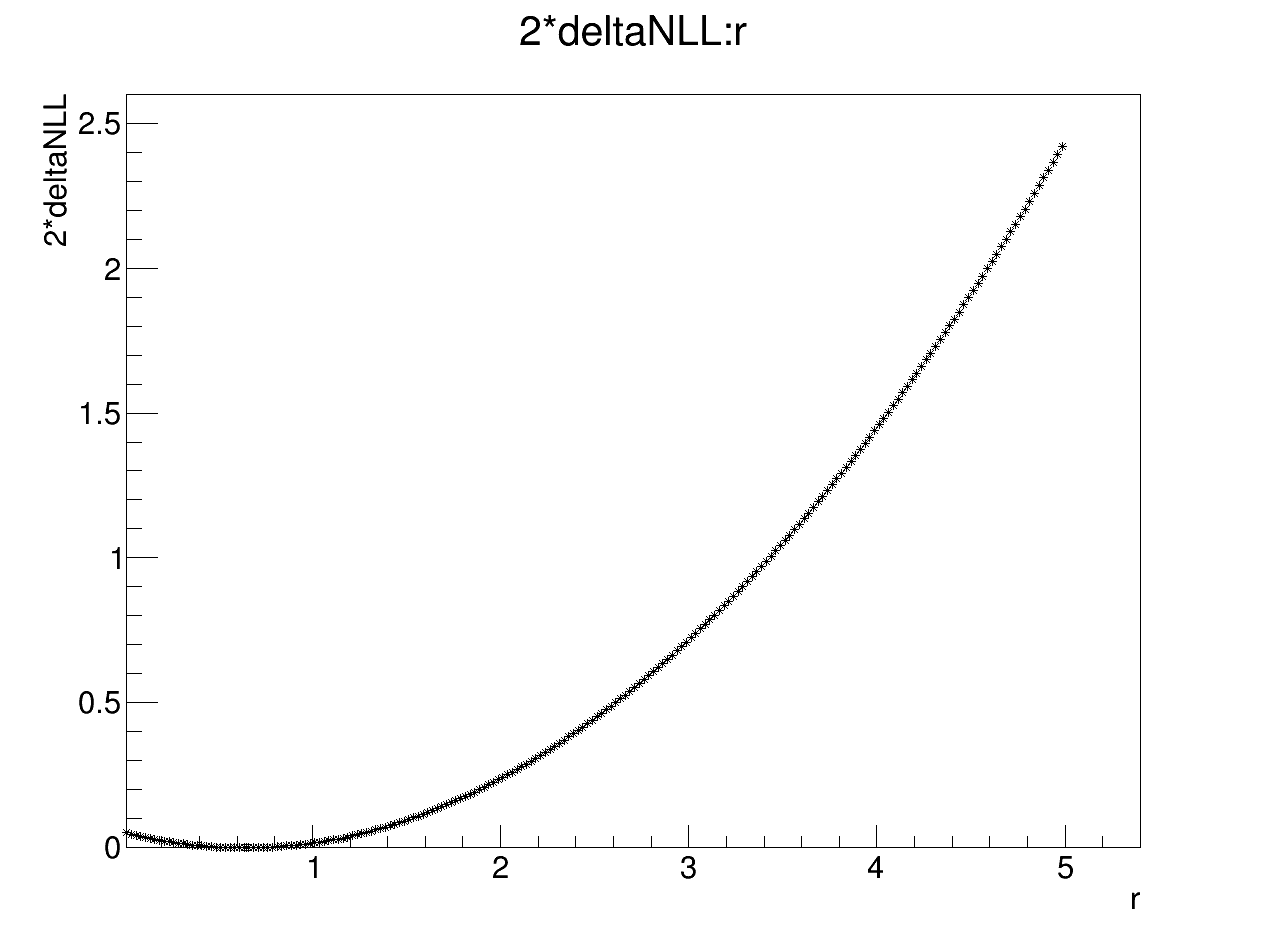
\includegraphics[width=0.3\textwidth]{figures/combine/asimovTests/NLL_asimovTest_1GeV.png}
     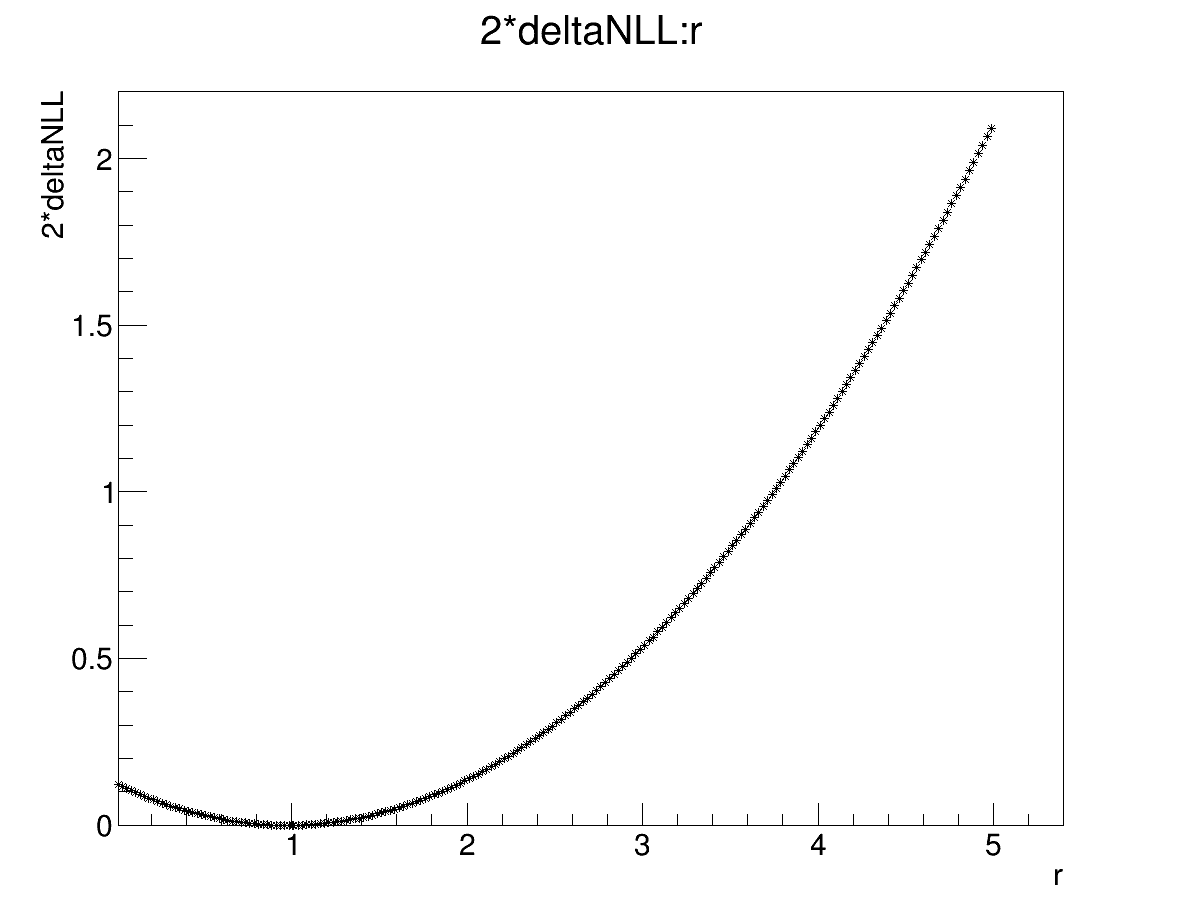
\includegraphics[width=0.43\textwidth]{figures/combine/asimovTests/NLL_asimovTest_p25GeV.png}
     \caption{The generated dataset dimuon mass spectrum overlaid with the extracted fit values (left). The
likelihood profiling vs. the injected signal strength r (right). }
     \label{combine:AsimovTests}
 \end{figure}

\subsection{Exclusion Limits}
The analysis is optimzed against the 95\% Confidence Level (CL) upper limits that we place on the SM production cross-section of the Higgs boson.
Expected limits are computed using the asymptotic approximation.

Figure~\ref{combine:LimitsAsymptotic} shows the expected exclusion limit computed using asymptotic approximation on the Asimov dataset
as a function of the probed Higgs boson mass and for the combination of all event categories as defined in Run~I analysis.

%The left plot shows limits for Higgs mass of $\mH=125\,\gev$ only but across all of the categories and various combinations.
%The right one shows exclusion limits as a function of the probed Higgs Mass and for a combination of all of the categories.

\begin{figure}[hbp]
     \centering
     %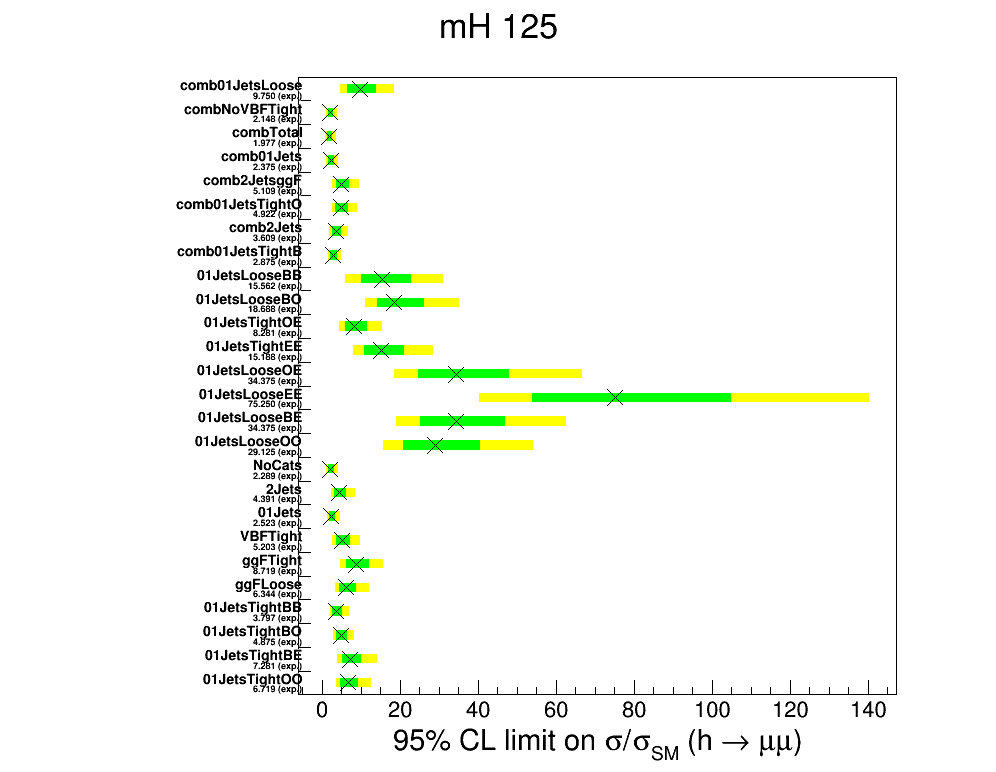
\includegraphics[width=0.45\textwidth]{figures/combine/limitsAsymptotic/baseline_110to160_p25GeV_NoNuis_Viktor/limitsByMass__125__TripleGaus.png}
      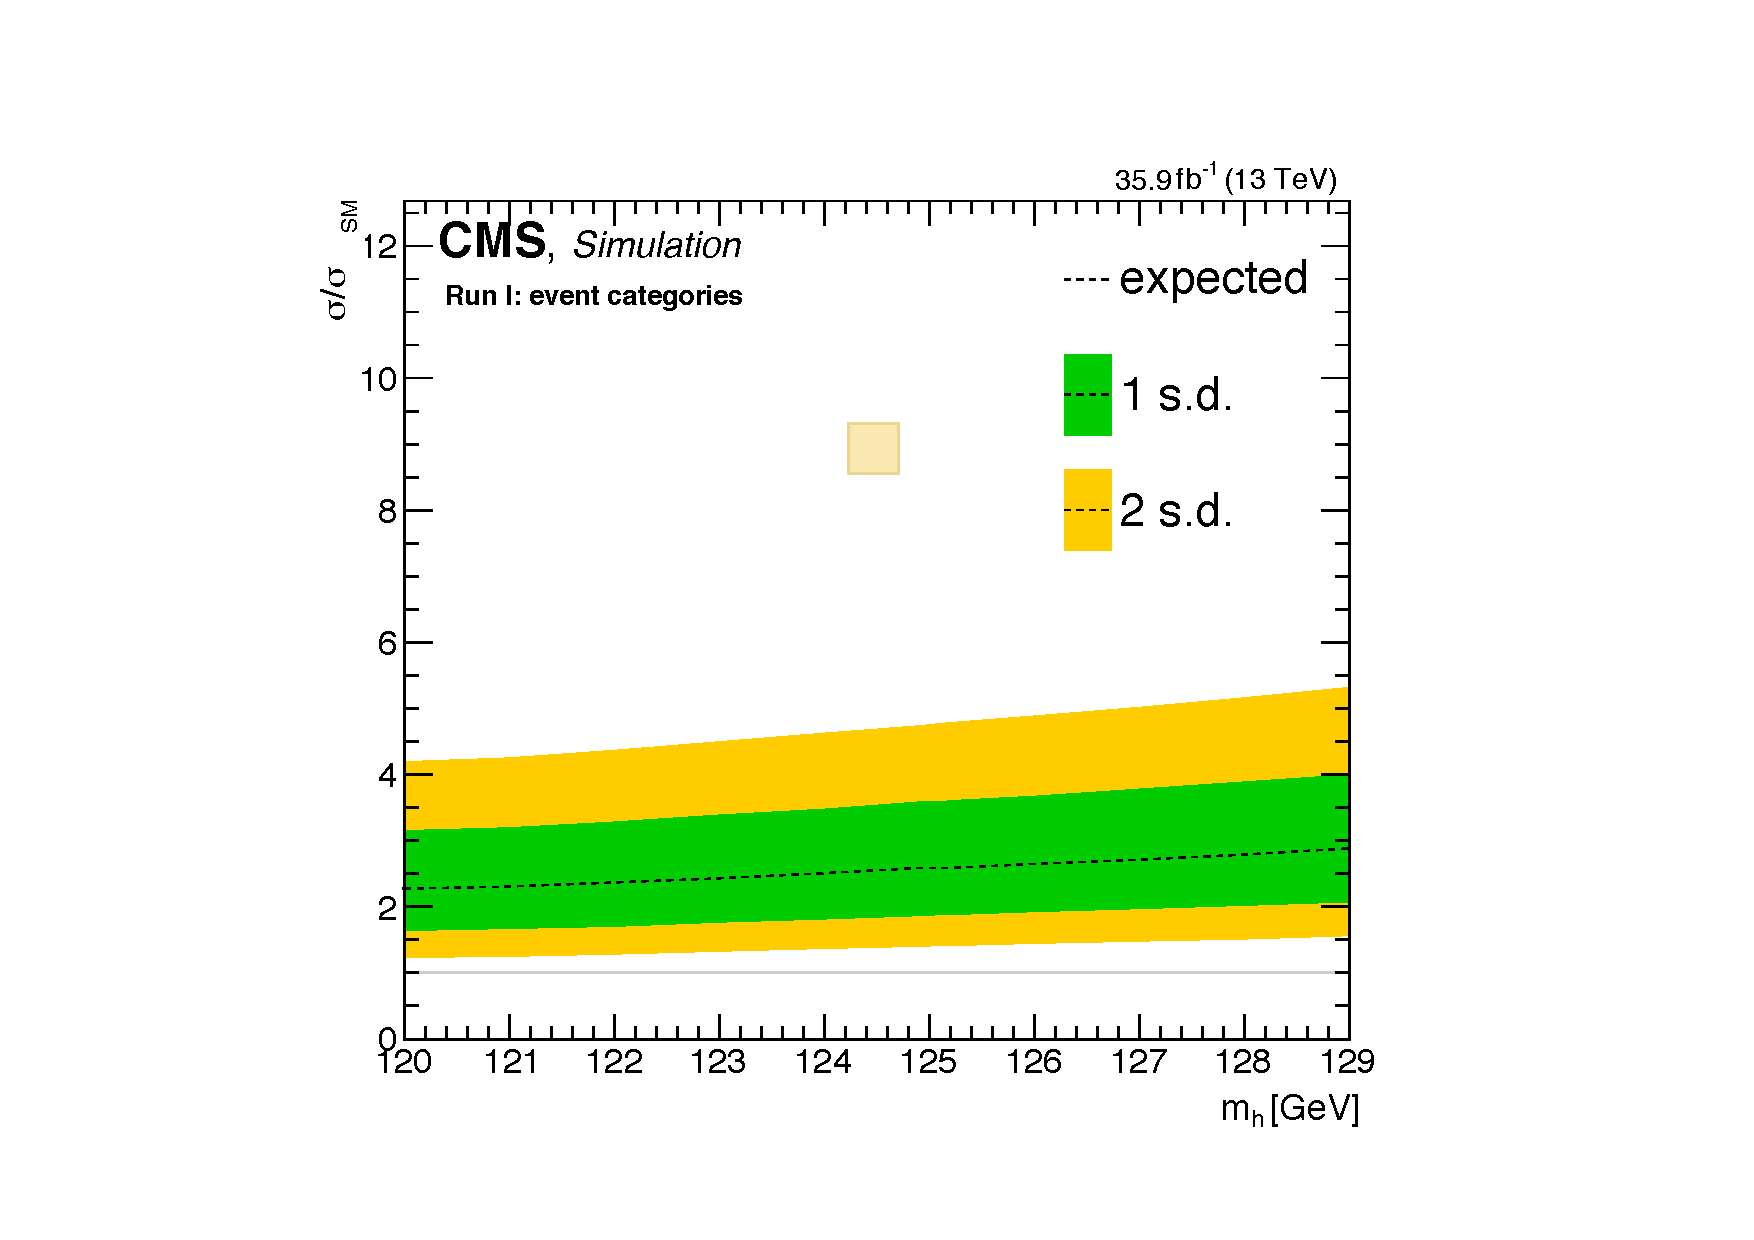
\includegraphics[width=0.8\textwidth]{figures/combine/limitsAsymptotic/baseline_110to160_p25GeV_NoNuis_Viktor/runIcat_b.pdf}
     \caption{The combined 95\% CL expected exclusion limit computed using asymptotic approximation as a function of the probed Higgs boson mass for event categories as defined in Run~I analysis. Only statistical uncertainties are considered.}
     \label{combine:LimitsAsymptotic}
 \end{figure}
